\documentclass[tikz]{standalone}
\usepackage{amsmath,amssymb}
\usepackage{pgfplots}

\pgfplotsset{compat=1.13}
\usepgfplotslibrary{fillbetween}

\begin{document}

 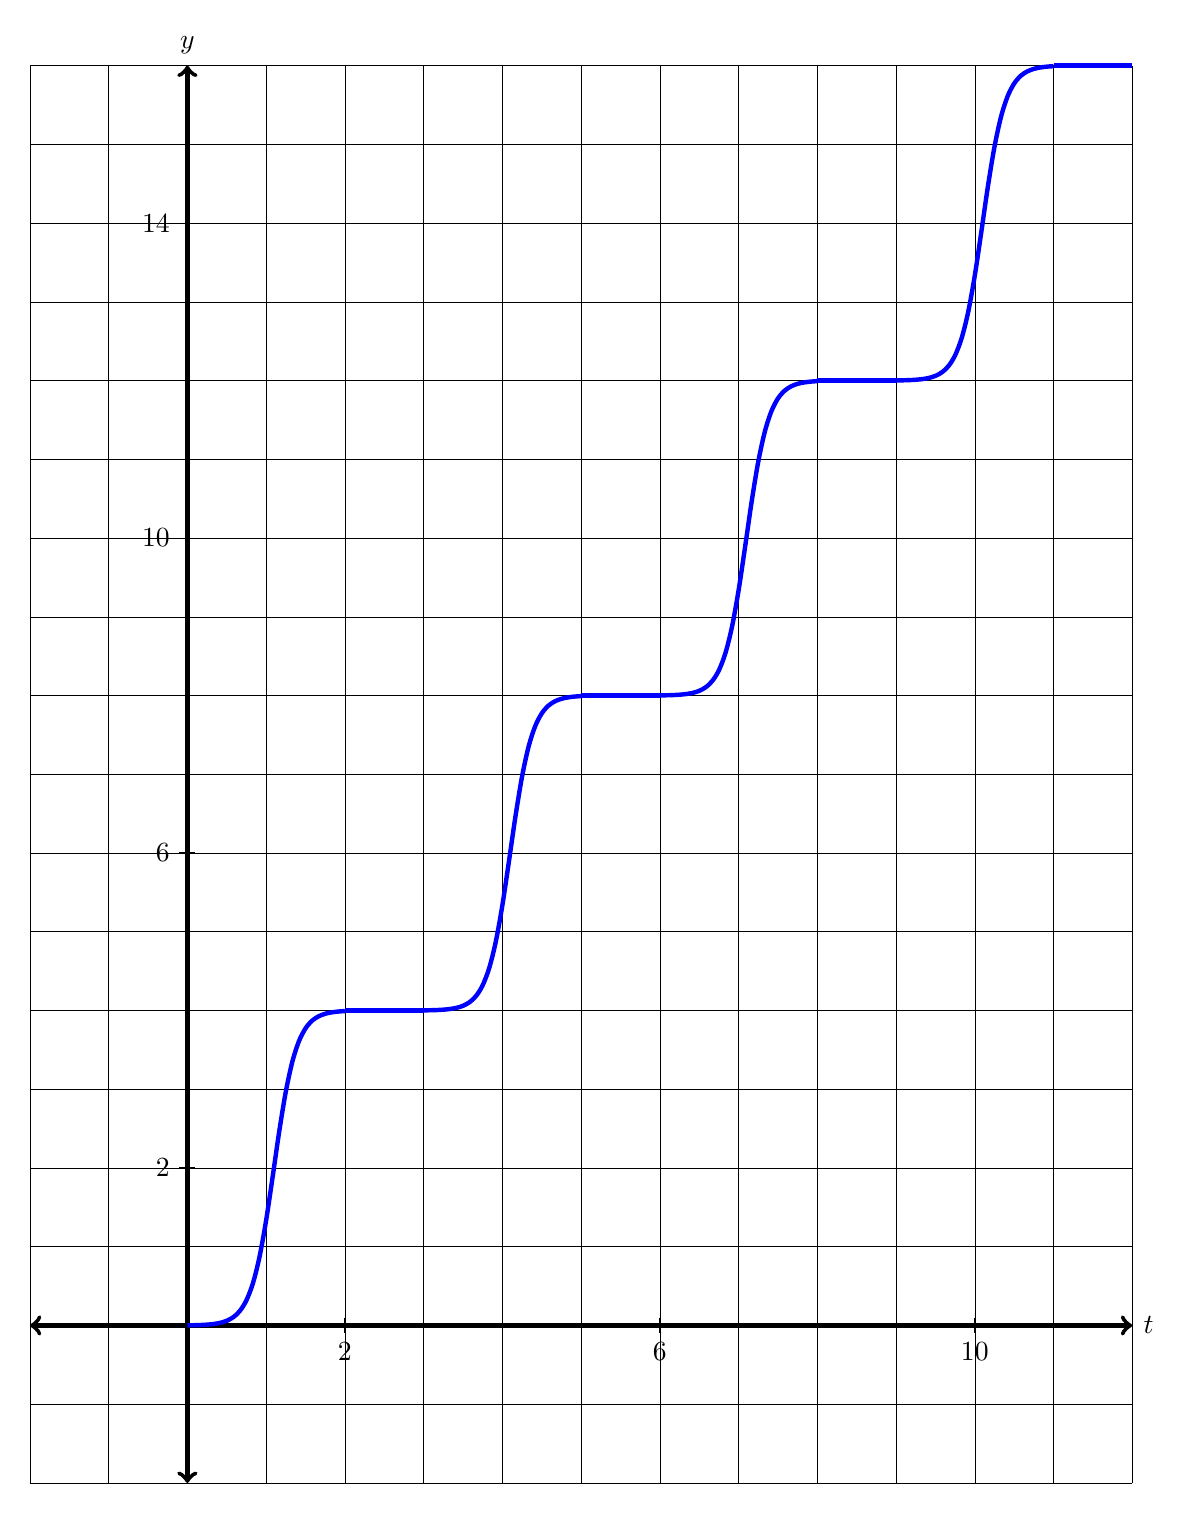
\begin{tikzpicture}[xscale=1,yscale=1]
 \draw[step=1.0,very thin] (-2,-2) grid (12,16);
        \draw[<->,ultra thick] (-2,0) -- (12,0) node[right] {$t$};
    \draw[<->,ultra thick] (0,-2) -- (0,16) node[above] {$y$};
	\foreach \x in {2,6,10} \draw (\x,0.1) -- (\x, -0.1) node[below] {\x};
	\foreach \y in {2,6,10,14} \draw (0.1,\y) -- (-0.1,\y) node[left] {\y};
	%\foreach \y in {-5,5} \draw (0.1,\y) -- (-0.1, \y) node[left] {\y};
	\draw[-,smooth,domain=0:2,very thick,blue, ultra thick] plot(\x,{4/(1+2*exp(-7*(\x-1)))});
	\draw[-,smooth,domain=2:3,very thick,blue, ultra thick] plot(\x,{4});
	\draw[-,smooth,domain=3:5,very thick,blue, ultra thick] plot(\x,{4/(1+2*exp(-7*(\x-4)))+4});
	\draw[-,smooth,domain=5:6,very thick,blue, ultra thick] plot(\x,{8});
	\draw[-,smooth,domain=6:8,very thick,blue, ultra thick] plot(\x,{4/(1+2*exp(-7*(\x-7)))+8});
	\draw[-,smooth,domain=8:9,very thick,blue, ultra thick] plot(\x,{12});
	\draw[-,smooth,domain=9:11,very thick,blue, ultra thick] plot(\x,{4/(1+2*exp(-7*(\x-10)))+12});
	\draw[-,smooth,domain=11:12,very thick,blue, ultra thick] plot(\x,{16});
\end{tikzpicture}
	
\end{document}
